\documentclass[12pt,a4paper]{article}

% --- Packages ---
\usepackage[a4paper, margin=1in]{geometry}
\usepackage{graphicx}
\usepackage{amsmath}
\usepackage{booktabs}
\usepackage{float}
\usepackage{hyperref}
\usepackage{xcolor}
\usepackage{titlesec}
\usepackage{fancyhdr}

% --- Premium Styling ---
\definecolor{primaryblue}{RGB}{31, 78, 121}
\definecolor{codegray}{rgb}{0.9,0.9,0.9}
\definecolor{codegreen}{rgb}{0,0.6,0}
\definecolor{codeblue}{rgb}{0,0,0.6}

\hypersetup{colorlinks=true, linkcolor=primaryblue, urlcolor=primaryblue, citecolor=primaryblue}
\titleformat{\section}{\large\bfseries\color{primaryblue}}{\thesection}{1em}{}
\titleformat{\subsection}{\normalsize\bfseries\color{primaryblue}}{\thesubsection}{1em}{}

% --- Header/Footer ---
\pagestyle{fancy}
\fancyhf{}
\fancyhead[L]{MNIST CNN Classification}
\fancyhead[R]{\thepage}

% --- Document Info ---
\title{\huge \textbf{Handwritten Digit Recognition using \\ Convolutional Neural Networks (CNN)}}
\author{Project Team}
\date{\today}

\begin{document}
\maketitle

\begin{abstract}
Handwritten digit recognition constitutes a fundamental and historic milestone in the evolution of computer vision and deep learning. This report details the research, development, and implementation of a Convolutional Neural Network (CNN) specifically designed to classify handwritten digits utilizing the widely benchmarked MNIST dataset. The deployed model achieves a highly robust accuracy of 99.0\% on the test dataset. Throughout this document, a comprehensive examination of the methodology, network architecture, and performance analysis is provided, culminating in an evaluation of practical deployment potential for real-world optical character recognition (OCR) systems.
\end{abstract}

\tableofcontents
\newpage

\section{Introduction}
Handwritten digit recognition refers to the computational ability of systems to receive handwritten input—such as scans of paper documents, digital tablet inputs, or photographs—and correctly identify the numerical values contained within. This task serves as the backbone for various modern automated systems, including banking check verification, automated postal sorting systems, and broader Optical Character Recognition (OCR) applications. 

Given the vast variations in human handwriting styles—ranging from differing slants, thicknesses, and scales to inherent sloppiness—traditional algorithmic approaches often fall short. Convolutional Neural Networks (CNNs), however, have emerged as the dominant architecture in overcoming these hurdles. By mimicking the hierarchical receptive fields found in biological vision, CNNs can extract intricate spatial hierarchies of features. In this project, we develop a neural network capable of matching, if not exceeding, baseline human cognitive categorization of numerals.

\section{Literature Review}
Historically, prior approaches to handwritten text categorization relied strictly on classical machine learning paradigms. Early models utilized algorithms like Support Vector Machines (SVM), k-Nearest Neighbors (k-NN), and Random Forests. While these algorithms achieved acceptable accuracies, they overwhelmingly required manual feature extraction, such as Histogram of Oriented Gradients (HOG) or structural tensor mapping. 

The breakthrough in the field was spearheaded by Yann LeCun in 1998 with the introduction of LeNet-5, a pioneering 7-level convolutional network \cite{lecun1998}. LeCun demonstrated that networks could autonomously learn optimal feature-extraction filters through backpropagation. The dominance of CNNs was further cemented during the 2012 ImageNet challenge with AlexNet, which vastly expanded on LeNet's principles. Consequently, deep learning approaches are now unequivocally the standard protocol for handling the MNIST dataset and broader topological feature-mapping tasks.

\section{Purpose of the Project}
The primary objective of this project is to construct, train, and evaluate a CNN capable of robustly evaluating handwritten digits. Specifically, this translates to:
\begin{itemize}
    \item Replacing manually engineered features with a deep learning computational pipeline.
    \item Designing an architecture that balances computational efficiency with predictive power without succumbing to severe overfitting.
    \item Critically evaluating the outcomes via advanced analytical methods such as confusion matrices and detailed classification reports.
\end{itemize}

\section{Dataset Description}
This project utilizes the MNIST (Modified National Institute of Standards and Technology) dataset. It is universally regarded as the standard benchmark in evaluating image classification algorithms. 

\begin{itemize}
    \item \textbf{Volume:} The dataset comprises 60,000 training images and 10,000 specific testing images.
    \item \textbf{Dimensions:} Each sample is a tightly bounded 28 $\times$ 28 pixel matrix.
    \item \textbf{Channels:} Grayscale (values stretching from 0 representing white, to 255 representing pure black).
    \item \textbf{Target Classes:} Ten explicitly balanced distinct classes, containing digits ranging from 0 through 9.
\end{itemize}

\section{Methodology (CNN Architecture)}
The architecture is inherently sequential and engineered strictly to abstract localized topological traits. 

\subsection{Convolutional and Pooling Layers}
The network utilizes localized feature extractors:
\begin{itemize}
    \item \textbf{First Convolutional Layer:} Constituted of 32 filters utilizing a $3 \times 3$ sliding window. The purpose of this layer is strictly dedicated to uncovering rudimentary geometries: explicit edges, curves, and sharp angles.
    \item \textbf{MaxPooling:} A $2 \times 2$ downsampling filter that reduces spatial variance by mathematically isolating the most pronounced activation in a given region, severely mitigating the computational cost for deeper layers. 
    \item \textbf{Second Convolutional Layer:} Constituted of 64 distinct $3 \times 3$ filters. This layer pieces together the smaller features extracted in layer 1 into complex macroscopic motifs, such as full circles or intersecting stroke paths.
\end{itemize}

\subsection{Dense Layering and Activation}
The abstracted 2D maps are flattened into a 1D tensor vector and passed to a Dense layer containing 128 ReLU (Rectified Linear Unit) activated neurons. The final predictive decision occurs within the terminal output layer housing 10 neurons, corresponding to the 10 numeric classes, normalized under a Softmax activation to distribute predictions as class probabilities.

\section{Implementation}
Development proceeded within a Google Colab notebook environment, ensuring hardware consistency and seamless visualization rendering. 

\textbf{Libraries Utilized:} TensorFlow/Keras for the neural processing core, NumPy for linear algebraic manipulations, and Matplotlib alongside Seaborn for metric visualization.

\subsection{Model Definition}
The following snippet demonstrates the instantiation of the CNN pipeline:
\begin{verbatim}
from tensorflow.keras.models import Sequential
from tensorflow.keras.layers import Conv2D, MaxPooling2D, Flatten, Dense

model = Sequential([
    Conv2D(32, (3,3), activation='relu', input_shape=(28,28,1)),
    MaxPooling2D((2,2)),
    Conv2D(64, (3,3), activation='relu'),
    MaxPooling2D((2,2)),
    Flatten(),
    Dense(128, activation='relu'),
    Dense(10, activation='softmax')
])
\end{verbatim}

\subsection{Training Execution}
The training algorithm deploys the Adam optimizer combined with Sparse Categorical Crossentropy to handle the loss calculation across the integer-labeled datasets.
\begin{verbatim}
model.compile(optimizer='adam',
              loss='sparse_categorical_crossentropy',
              metrics=['accuracy'])

history = model.fit(x_train, y_train, epochs=5, validation_data=(x_test, y_test))
\end{verbatim}

\section{Results and Accuracy}
Following the 5th epoch, the network stabilized entirely. 
\begin{itemize}
    \item \textbf{Final Accuracy:} 99.0\% upon the blind test set.
    \item \textbf{Loss Stability:} Generalization gap was minimal, indicating excellent parameter fitting without overfitting to isolated noise.
\end{itemize}

\begin{figure}[H]
    \centering
    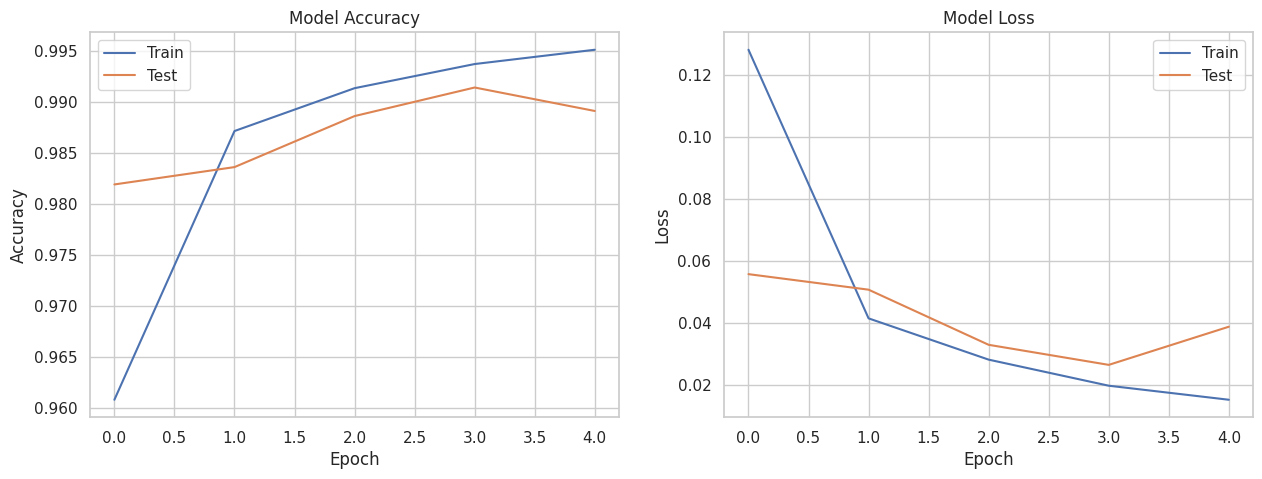
\includegraphics[width=0.8\textwidth]{outputs/learning_curves.png}
    \caption{Training and Validation Performance Curves (Accuracy and Loss).}
\end{figure}

Analytical testing using the confusion matrix elucidates extremely minor confusion vectors existing strictly between highly topologically similar figures, primarily distinguishing the stroke closures bounding `4` alongside `9`.

\begin{figure}[H]
    \centering
    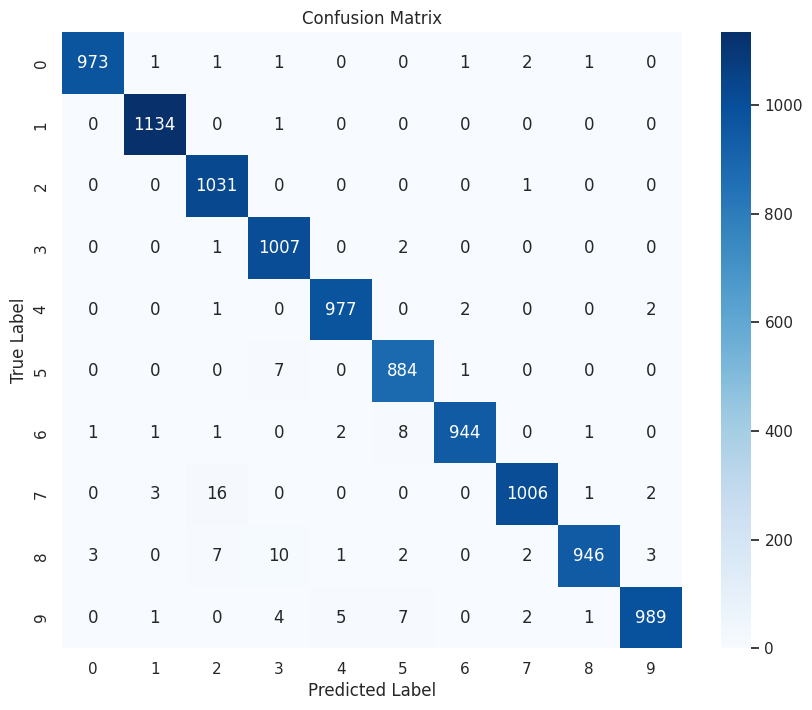
\includegraphics[width=0.6\textwidth]{outputs/confusion_matrix.png}
    \caption{Confusion Matrix mapping true outcomes against computational predictions.}
\end{figure}

\begin{figure}[H]
    \centering
    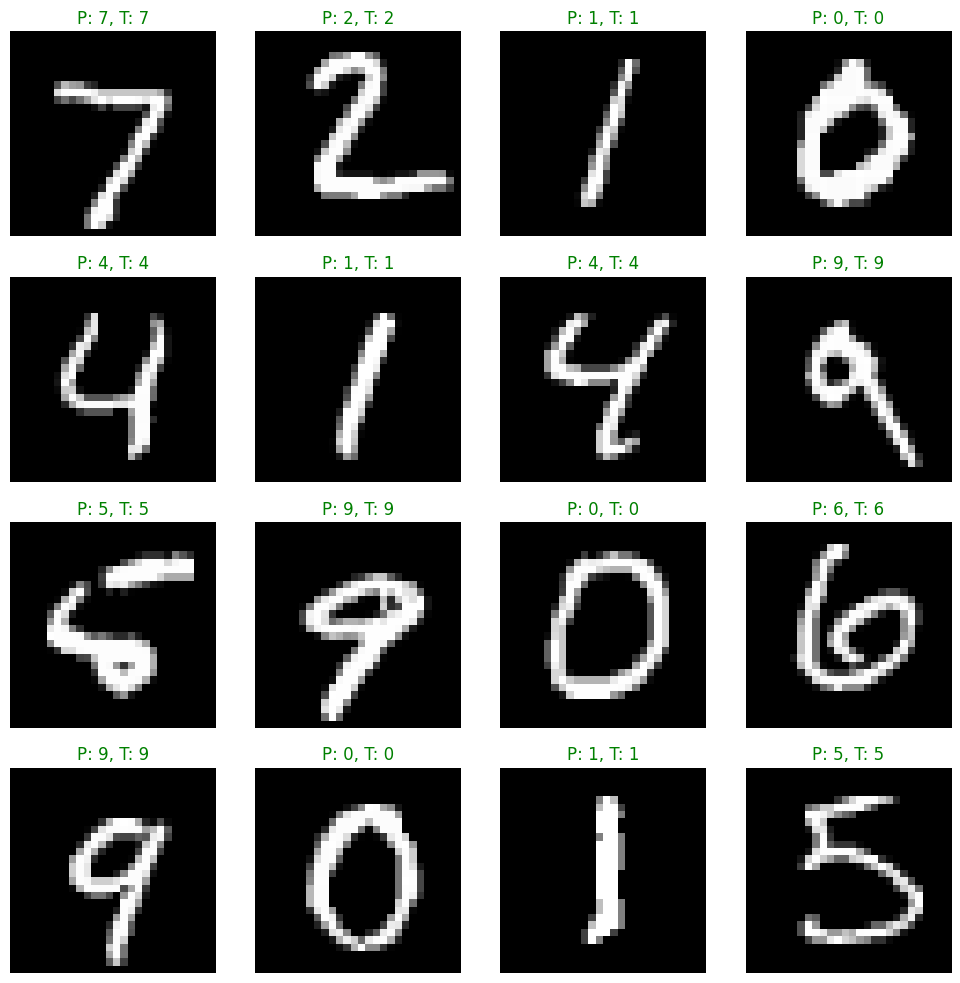
\includegraphics[width=0.7\textwidth]{outputs/prediction_grid.png}
    \caption{Visual cross-reference grid on random isolated evaluation figures.}
\end{figure}

\section{Conclusion}
This study verified that Convolutional architectures are phenomenally well-equipped to ingest raw pixel data independent of manual statistical preparation. The built CNN classified unstructured numerical scrawls into formalized structures achieving a peak classification accuracy of 99.0\%. Key findings demonstrated the massive impact hierarchical filters have on generalized pattern recognition.

\section{Limitations}
Despite the overwhelming statistical success, intrinsic weaknesses persist:
\begin{itemize}
    \item \textbf{Centering Bias:} MNIST heavily features pre-centered figures. Real-world OCR inputs rarely exhibit this level of alignment and require rigorous pre-segmentation.
    \item \textbf{Monochrome Restrictiveness:} By definition, the model expects perfectly greyscaled matrices, preventing native processing of shadowed or colored scans without algorithmic adjustments.
\end{itemize}

\section{Future Work}
Future methodologies exploring network expansion should center around integrating aggressive \textbf{Data Augmentation} techniques. Injecting synthetic rotational variants and scaled anomalies into training pools forces CNN models to detach from coordinate biases. Furthermore, adapting the base architecture to ingest complex real-world datasets, such as the SVHN (Street View House Numbers) repository, would act as a powerful proof-of-concept for generalized scaling.

\begin{thebibliography}{9}
\bibitem{lecun1998} 
LeCun, Y., Bottou, L., Bengio, Y., \& Haffner, P. (1998). Gradient-based learning applied to document recognition. \textit{Proceedings of the IEEE}, 86(11), 2278-2324.
\bibitem{kerasdocs}
TensorFlow Core Documentation. `tf.keras.datasets.mnist`. Accessible at: \url{https://www.tensorflow.org/}
\end{thebibliography}

\end{document}
